%!TEX root = tesis.tex


\chapter{Un \ssolver paralelo y distribuido }
\label{ssolver-pardist}

La implementación de nuestra herramienta como un sistema distribuido persigue
el objetivo fundamental de mejorar el tiempo de ejecución ya sea decrementando
el tiempo necesario para resolver un determinado problema o transformando un
problema previamente irresoluble (en tiempo razonable) en resoluble. Para ello
el sistema debe ser \textbf{escalable} en tanto que debe tener la capacidad de
incorporar mayor cantidad de \hard a la resolución del problema. Por otro
lado, el uso de este \hard debe ser \textbf{eficiente} en el sentido de que la
utilización de mayor cantidad de \hard debe resultar en un incremento de la
performance del sistema (en nuestro caso entendida como se describió
previamente).

Con estos dos objetivos en mente desarrollamos una \ssolver distribuido basado
en la idea de \gp y orienteado a \clusters de computadoras. La idea de \gp se
basa en la observación de que, en el peor caso, todas las posibles valuaciones
de una fórmula proposicional $\varphi$ deben ser evaluadas de modo de poder
concluir que la misma es \unsat. Por lo tanto, una forma de dividir el
problema es tomar una variable $v$ y construir los dos subproblemas
$\varphi_{v \leftarrow 0}$ y $\varphi_{v \leftarrow 1}$ que se derivan de las
dos posibles asignaciones de valores de verdad a dicha variable. Una vez hecho
esto, la resolución del problema original $\varphi$ se reduce a la resolución
de $\varphi_{v \leftarrow 0}$ y $\varphi_{v \leftarrow 1}$. Ahora, $\varphi_{v
\leftarrow 0}$ y $\varphi_{v \leftarrow 1}$ pueden ser considerados como dos
problemas independietes y volver a aplicar la misma idea. Naturalmente este
proceso puede realizarse seleccionando más de una variable en cada paso. Al
seleccionar $n$ variables obtendremos entonces $2^n$ subproblemas. Llamaremos
\emph{levantar variables} al proceso de dividir un problema $\varphi$ en los
$2^n$ subproblemas que resultan de aplicar todas las posibles valuaciones
sobre el conjunto de $n$ variables levantadas. Se desprende de esto que una de
las tareas que debe poder cumplir la herramienta es la de dividir un problema.

\missingfigure{Un dibujito que explique \gp}

% El objetivo principal de todo sistema distribuido es que el mismo sea
% \textbf{escalable}. Si bien la escalabilidad puede ser entendidad en
% diferentes sentidos, nos interesa en particular que el sistema haga posible la
% utilización de mayor cantida de \hard para resolver el problema (en nuestro
% caso un problema \sat) y que esa utilización de mayor poder de cómputo reporte
% ganancias en términos de tiempo (percibido) invertido en resolver un
% determinado problema o bien en términos de empujar la frontera de lo
% resoluble.

La escalabilidad como gran objetivo rector en el desarrollo de nuestra
herramienta introduce una serie de desafíos a saber:
\begin{itemize}
	\item Almacenamiento distribuido.
	\item Simetría de capacidades en los nodos de trabajo (\ws).
	\item Minimización de la utilización de la red de comunicaciones.
\end{itemize}

La necesidad de que el almacenamiento de problemas pendientes de resolución se
encuentre distribuido se debe a un doble aspecto. Por un lado, la cantidad de
subproblemas producidos puede ser muy grande. Por lo tanto no es viable
requerir que la cantidad de espacio necesario para almacenar todas las tareas
pendientes de resolución se encuentre disponible en una misma ubicación. Aún
cuando fuera posible tener la cantidad de espacio necesaria para almacenar
todos los subproblemas en una ubicación centralizada surge un segundo problema
que presentaría este enfoque que es el de la contención. En este aspecto, si
pretendemos que el almacenamiento no se vuelva un cuello de botella es vital
distribuir de la mejor manera posible las tareas pendientes de modo que cuando
los \ws requieran nuevas tareas para resolver, los múltiples pedidos no
recaigan en un mismo equipo.

El requisito de que los nodos de trabajo (\ws) sean símetricos se desprende de
la necesidad de eliminar los cuellos de botella. La simetría entendida en su
máxima expresión como la posibilidad de que todas las unidades de
procesamiento puedan realizar todas las funciones necesarias provee la
capacidad de distribuir la carga de trabajo de la manera más conveniente en
cada momento. Esto no podría ser logrado si los nodos de trabajo tuvieran
funciones específicas ya que se podría dar el caso de tener nodos ociosos
porque no hay trabajo pendiente de la clase de trabajo que esos nodos saben
realizar mientras que al mismo timepo tendríamos nodos sobrecargados. Esta
situación podría empeorar seriamente a medida que la cantidad de nodos
aumenten.

En nuestro caso particular, el requisito de simetría se traduce en que los \ws
deben poseer las capacidades de: \begin{inparaenum}[a)] \item \solvear
\todo{buscar una forma de decir esto que no sea tan fea o en su defecto
definir esto en la parte de preliminares} un subproblema (consumir), \item
dividir un subproblema en nuevos subproblemas (producir) y \item almacenar,
solicitar y transferir subproblemas (distribuir). \end{inparaenum}

Además de los desafíos de escalabilidad, surgen también los desafíos
relacionados con la eficiencia o la performance de la herramienta. Entre ellos
los más destacados son:

\begin{itemize}
	\item Movilidad de tareas.
	\item Crecimiento a la par de los \ssolvers secuenciales.
	\item No hacer burradas \todo{Revisar toda esta itemización. No me convence....}
\end{itemize}

El triple rol de productor, consumidor y distribuidor asignado a los \ws hace
que la movilidad de tareas se transforme en un desafío en tanto que un \w
puede estar \solveando al mismo tiempo que otro \w le solicita una tarea
pendiente. Es evidente que en esta situación no es viable que el \w que está
esperando una tarea tenga que esperar a que el \w que tiene dicha tarea
termine de \solvear para que su pedido sea completado.

Otro de los objetivos que perseguimos a la hora de diseñar nuestra herramienta
fue que la misma pudiera utilizar un \ssolver \ots para la resolución local de
un subproblema. Esto nos permite aprovechar los avances que se han obtenido en
el área de \ssolving secuencial en los últimos años (que han sido muchos) a la
vez que nos permite, a futuro, evolucionar a la par de los \ssolvers
secuenciales de manera más simple. Esto proporciona la posibilidad de que la
herramienta no se vuelva obsoleta ante un nuevo avance en el campo de
\ssolving secuencial.

\newcommand{\rt}{\emph{run-time}\xspace}
\newcommand{\apriori}{\emph{a priori}\xspace}

Generar una estrategia automática que proporcione buenos resultados en la
ejecución de problemas diversos es sumamente difícil. Más aún, no tener la
posibilidad de modificar la estrategia adoptada durante una corrida (que puede
ser sumamente larga y con características desconocidas \apiori) puede tener
resultados catastróficos. Esto nos motivó a adoptar un enfoque en el que la
maquinaria de cómputo distribuido no posee inteligencia alguna y por el
contrario provee una serie de funciones básicas que pueden ser invocadas
remotamente. La operación del sistema por lo tanto se lleva a cabo desde un
\textbf{tablero de control} que permite al usuario manipular el sistema de
cómputo en \rt.

\

\noindent\underline{\textbf{Nota sobre la implementación}}

\

El último objetivo que perseguimos durante el desarrollo de nuestra
herramienta fue que la misma presentara facilidad para ser modificada sin que
esto impacatar negativamente en la \emph{performance}. Este objetivo, entre
otras cosas, determinó la elección de las tecnologías a utilizar para su
desarrollo. Por lo tanto se utilizó el lenguaje de programación \Python para
el desarrollo de toda la herramienta con excepción de la parte de cómputo
intensivo. Al utilizar un \ssolver \ots no fue necesario elegir un lenguaje
para su desarrollo. En la implementación actual de la herramienta utilizamos
el \ssolver \minisatdosveinte que está desarrollado en el lenguaje \cpp. Para
ello se desarrolló un \emph{wrapper} que permite utilizar \minisat desde un
entorno \Python. Para el intercambio de mensajes entre los \ws se utilizó el
estándar \mpi.


% \begin{itemize}
% 	\item Escalable
% 	\item Uso de SAT Solver off-the-shelf
% 	\item Multiplataforma
% 	\item Tablero de control
% \end{itemize}

\section{Arquitectura}

\newcommand{\fig}{Fig.-}

La \fig\ref{fig:arquitectura} muestra la arquitectura de la herramienta. En
la misma se distinguen claramente dos componentes: el \bend que ejecuta sobre
un \cluster de computadoras y el \fend que ejecuta en un equipo que se
encuentra posiblemente fuera del centro de cómputos.

\begin{wrapfigure}{R}{0.4\textwidth}
\label{fig:arquitectura}
\fbox{\includegraphics[scale=0.4]{graphs/paralloy architecture}}
\caption{Diagrama de componentes y conectores del \ssolver distribuido}
\end{wrapfigure}

\subsection{\bend}

\newcommand{\master}{\emph{MasterProxy}\xspace}

En el \bend se puede observar que existen dos clases distintas de elementos.
Por un lado tenemos un proceso llamado \master que es el encargado de manejar
la comunicación de órdenes desde el \fend hacia los \ws y de reenviar las
respuestas correspondientes desde los \ws hacia el \fend.

En segunda instancia encontramos otro de tipo de procesos, los \ws. Los \ws
son los encargados de relizar el cómputo (\ssolving) y la división de un
problema en nuevos subproblemas. Asimismo son quienes almacenan las tareas
pendientes de ejecución y por lo tanto deben proveer acceso a dicho
almacenamiento a los demás \ws.

\newcommand{\masterslave}{\texttt{Master-Worker}\xspace}

Es importante destacar que si bien el \bend presenta una arquitectura
\masterslave, el \master en este caso no toma ninguna decisión sino que
simplemente actúa como intercambiador de mensajes entre el ambiente externo
(el \fend) y el ambiente interno.

\begin{wrapfigure}{O}{0.85\textwidth}
\centering
\includegraphics[scale=0.3]{graphs/master proxy detail}
\caption{Detalle de arquitectura del componente \master}
\label{fig:masterproxydetail}
\end{wrapfigure}

La \fig\ref{fig:masterproxydetail} detalla la arquitectura del \master. En el
diagrama se puede observar que el \datapath de entrada (\fend hacia \bend) y
el de salida (\bend hacia \fend) son independientes. Esto es una consecuencia
directa que se desprende de la ausencia de inteligencia en el \master. Esto
implica que no es necesario mantener el estado del sistema ya que en este
componente no se toman decisiones. La ausencia de estado hace que el proceso
\master consuma un mínimo de recursos.

La intervención de dos \threads distintos en el \datapath de entrada
proporciona un alto nivel de respuesta ya que permite que algunos comandos
sean implementados internamente mediante comunicación sincrónica a través de
\mpi sin que esto implique una pausa en el procesamiento del flujo de datos de
entrada desde el \fend hacia el \bend. La comunicación sincrónica permite
simplificar algunos comandos como el envío del problema original hacia todos
los \ws. Al mismo tiempo se mantiene el orden entre los comandos enviados
desde el \fend lo cual también contribuye a la simplifación del modelo de
cómputo a pesar de tratarse de un sistema ditribuido.

\begin{wrapfigure}{O}{0.75\textwidth}
\centering
\includegraphics[scale=0.3]{graphs/worker detail}
\caption{Detalle de arquitectura del componente \w}
\label{fig:workerdetail}
\end{wrapfigure}

La \fig\ref{fig:workerdetail} muestra el detalle de diseño del componente
\w. Como se puede observar, las funciones de \solving, comunicación y
transferencia de archivos se implementaron en \threads separados. Dado que la
función de \solving utiliza principalmente tiempo de \cpu, mientras que el
resto de las funciones consumen principalmente timepo de \io, la separación de
éstas en distintos \threads permite la ejecución concurrente de estas
tareas sin que esta característica impacte negativamente en el desempeño del
\ssolver. A la vez, esta característica permite satisfacer el objetivo de
movilidad de las tareas, aún cuando el \w se encuentre ocupado \solveando.

Interesa destacar también que tanto la estrategia de partición de un problema
como la estrategia de aprendizaje se encuentran implementadas en los \ws. Si
bien este diseño es contrario a la idea general de \emph{tablero de control}
consideramos que el nivel de granularidad necesario para poder controlar
remotamente la realización de estas dos tareas era demasiado alto y atentaba
contra la usabilidad de la herramienta. Asimismo, la herramienta es capaz de
poseer diversas estrategias implementadas para estas dos fases de la ejecución
de modo que el usuario puede seleccionar la estrategia deseada (y sus
parámetros en caso que corresponda) desde el \fend.

\subsection{\fend}

bal ablablmas
kiasdoil
asdk.jasd
ñljasd


\begin{figure}
	\begin{subfigure}[b]{0.5\textwidth}
		\centering
		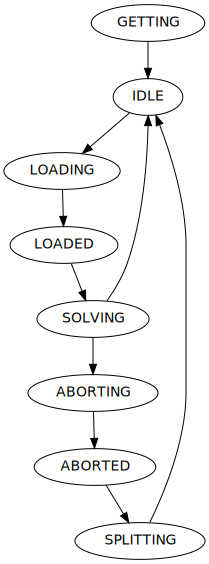
\includegraphics[scale=0.5]{graphs/workerstates}
		\caption{\emph{Workers}}
	\end{subfigure}
	\begin{subfigure}[b]{0.5\textwidth}
		\centering
		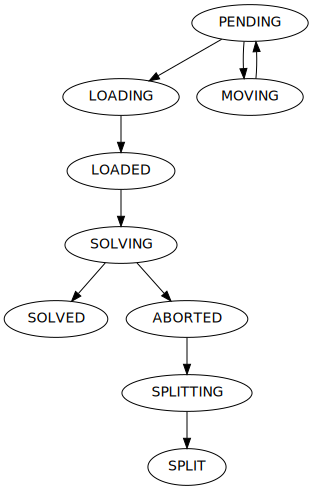
\includegraphics[scale=0.5]{graphs/taskstates}
		\caption{Tareas}
	\end{subfigure}
	\caption{Diagramas de estado en el tablero de control}
\end{figure}

la interfaz de la estrategia


\begin{wrapfigure}{O}{.6\textwidth}
\begin{tiny}
\begin{lstlisting}[language=Python,caption=Interfaz Strategy]
class Strategy(object):
	def register_globalstate(self, globalstate)
	def register_socket(self, commandsocket)
	def on_init(self, worker)
	def on_createroot(self, worker, task)
	def on_init_finished(self, nworkers)
	def on_getfile(self, worker, task)
	def on_file(self, worker, task)
	def on_load(self, worker, task)
	def on_unsat(self, worker, task)
	def on_sat(self, worker, task, modelstr)
	def on_abort(self, worker, task)
	def on_split_newtask(self, worker, newtask)
	def on_split_finished(self, worker, parenttask, nchildren)
	def on_shutdown(self)
\end{lstlisting}
\end{tiny}
\end{wrapfigure}

\subsection{Nuestra estrategia}

\begin{itemize}
	\item Si idle se parte el más viejo
	\item La próxima a resolver es:
		\begin{itemize}
			\item Si no tengo tareas locales:
				\begin{itemize}
					\item Bajo la tarea que corresponde por BFS +
					\item $\frac{\sharp tasks}{\sharp workers}$ del que más tiene (límite 10)
				\end{itemize}
			\item Si tengo: Agarro la que corresponde por BFS
		\end{itemize}
	\item Parto cuando la frecuencia de $\sharp UNSATs/_s$
	\item Detalles:
	\begin{itemize}
		\item Target de UNSATs por esgundo
		\item Frecuencia de checkeo
		\item Tamaño ventana
	\end{itemize}
\end{itemize}

\subsection{Decisiones que vale la pena seguir investigando}

\section{Resultados experimentales}

\begin{table}[h]\tiny
	\begin{tabular}{lrrrrrr}
		\toprule
		problem	&	scope	&	sequential runtime	&	parallel walltime	&	parallel overhead	&	speedup	&	efficiency \\
		\cmidrule(r){1-7}
		Pamela	&	8	&	308.26	&	60.46	&	3561.23	&	5.10x	&	0.08 \\
		Pamela	&	9	&	76168.16	&	407.34	&	-50098.63	&	186.99x	&	2.92 \\
		Pamela	&	10	&		&		&	0.00	&		&	 \\
		\cmidrule(r){1-7}
		Closure	&	11	&	749.65	&	291.28	&	17891.95	&	2.57x	&	0.04 \\
		Closure	&	12	&	3983.36	&	1914.45	&	118541.30	&	2.08x	&	0.03 \\
		Closure	&	13	&		&		&	0.00	&		&	 \\
		\cmidrule(r){1-7}
		MarkGC Soundness2	&	9	&	217.31	&	200.85	&	12637.31	&	1.08x	&	0.02 \\
		MarkGC Soundness2	&	10	&	2855.3	&	1376.89	&	85265.47	&	2.07x	&	0.03 \\
		\bottomrule
	\end{tabular}
	\caption{Tiempo de ejecución (en segundos) distribuido vs. secuencial}
	\todo[inline]{Resultados parciales. Completar con todos los experimentos}
\end{table}